\documentclass[10pt]{article}
\usepackage[margin=1in]{geometry}
\usepackage{graphicx}
\usepackage{amsmath,amssymb}
\usepackage{hyperref}
\usepackage{booktabs}
\usepackage{longtable}
\usepackage{caption}
\captionsetup{labelfont=bf,font=small}
\graphicspath{{NHB_Symbolic_Mainfold/code/figs_final/}{./}}

\title{Supplementary Information for\\
\emph{Symbolic Manifolds and Entropic Dynamics: A Computational Framework for Monitoring Cognitive Network Recovery in Regenerative Medicine}}
\date{}

\begin{document}
\maketitle

\section*{Mathematical Notes}

\subsection*{Entropy rate}
Let $X_1,X_2,\dots$ be a stationary Markov chain on a finite set with transition matrix $P$. The entropy rate is
\begin{equation}
H_{\mathrm{rate}}(P)=-\sum_{i}\pi_i\sum_{j}P_{ij}\log P_{ij},
\end{equation}
where $\pi$ is the stationary distribution ($\pi^\top P=\pi^\top$). Logs are natural unless otherwise stated.

\subsection*{Transition operator with entropic control}
Given edge weights $W_{ij}\ge 0$ on a directed graph, define
\begin{equation}
P_{ij}(\beta)=\frac{W_{ij}^{\,\beta}}{\sum_{k}W_{ik}^{\,\beta}},\qquad \beta\ge 0,
\end{equation}
which interpolates from maximally exploratory ($\beta=0$) to focused dynamics ($\beta\to\infty$). Under mild conditions, $P(\beta)$ is ergodic with unique stationary distribution $\pi(\beta)$.

\subsection*{Ollivier--Ricci curvature}
For nodes $u,v$ with distance $d(u,v)$ and neighbourhood measures $\mu_u,\mu_v$ (with anchoring $\alpha\in[0,1]$), the edge curvature is
\begin{equation}
\kappa_{\mathrm{OR}}(u,v)=1-\frac{W_1(\mu_u,\mu_v)}{d(u,v)},
\end{equation}
where $W_1$ is the 1-Wasserstein distance. We use $\mu_x=\alpha\delta_x+(1-\alpha)\,\mathrm{Unif}(\mathcal{N}(x))$, with $\alpha=0.5$ unless noted. Forman curvature is reported as a sensitivity check.

\subsection*{Lemma (monotonicity of $H_{\mathrm{rate}}$ in $\beta$)}
For the family $P(\beta)$ above, $H_{\mathrm{rate}}(\beta)$ is non-increasing in $\beta$, with maximum at $\beta=0$ and $H_{\mathrm{rate}}(\beta)\to 0$ as $\beta\to\infty$ when transitions become deterministic. \emph{Sketch:} the conditional entropy $H[P_{i\cdot}(\beta)]$ decreases with $\beta$ by concavity of entropy as probability mass concentrates; averaging by $\pi(\beta)$ preserves monotonicity.

\section*{Glossary (selected terms)}
\begin{longtable}{@{}p{3cm}p{12cm}@{}}
\toprule
Entropy rate & Average information per step of a stationary stochastic process; for a Markov chain, weighted average of row entropies.\\[3pt]
Ollivier--Ricci curvature & Graph-geometric quantity comparing neighbourhood overlap via optimal transport; negative values concentrate on bridges/bottlenecks.\\[3pt]
Configuration model & Degree-preserving random graph used as a null model.\\[3pt]
Trustworthiness/Continuity & Metrics assessing local/global faithfulness of embeddings (reported for PCA/t-SNE/UMAP).\\
\bottomrule
\end{longtable}

\section*{Table of Symbols}
\begin{longtable}{@{}p{3cm}p{10cm}p{3cm}@{}}
\toprule
Symbol & Meaning & Unit/Scale\\ \midrule
$H_{\mathrm{rate}}$ & Entropy rate of the Markov chain & nats/step \\
$\kappa_{\mathrm{OR}}$ & Ollivier--Ricci curvature (edge-averaged unless noted) & dimensionless\\
$P(\beta)$ & Transition matrix with entropic control & probability rows\\
$\beta$ & Bias (inverse-temperature) parameter & dimensionless\\
$\alpha$ & Anchoring parameter for curvature transport & dimensionless\\
$E_{\mathrm{glob}}$ & Global efficiency & dimensionless\\
$Q$ & Modularity (directed extension) & dimensionless\\
\bottomrule
\end{longtable}

\section*{Additional Figures}

\begin{figure}[H]\centering
\includegraphics[width=\linewidth]{Fig_gamma_profiles.pdf}
\caption{\textbf{Supplementary Fig. S1 | Regime profiles across the symbolic manifold.} Latent activation profiles for simulated regimes; shaded areas indicate variability across seeds.}
\end{figure}

\begin{figure}[H]\centering
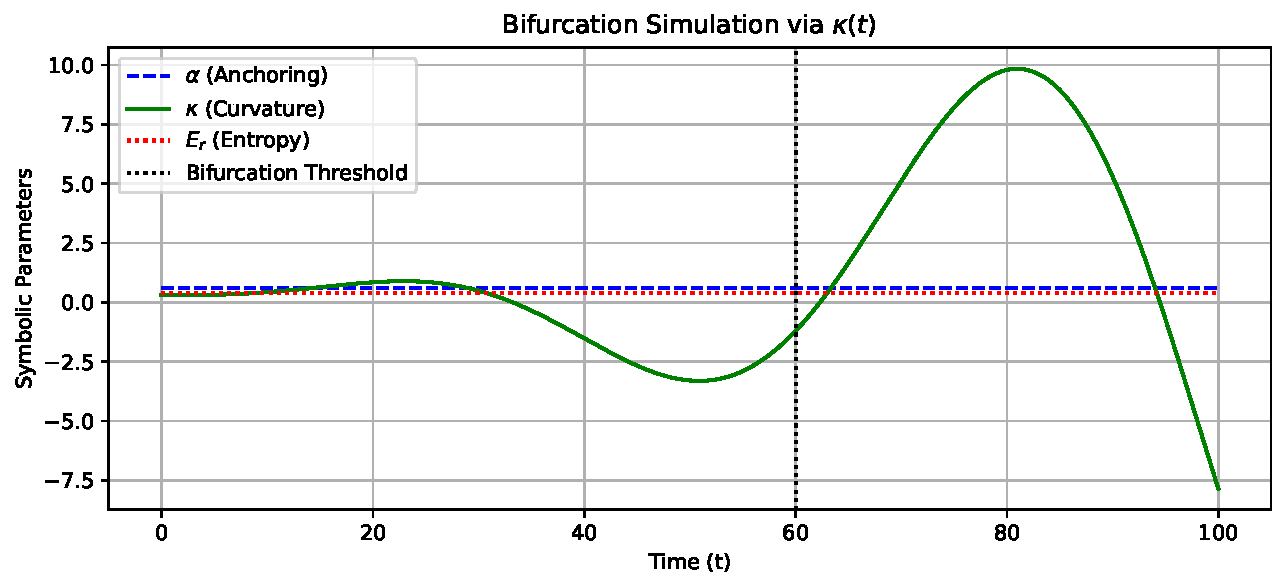
\includegraphics[width=\linewidth]{Fig_kappa_bifurcation.pdf}
\caption{\textbf{Supplementary Fig. S2 | $\kappa$-bifurcation schematic.} Steady-state response as a function of curvature control, illustrating regime transitions.}
\end{figure}

\begin{figure}[H]\centering
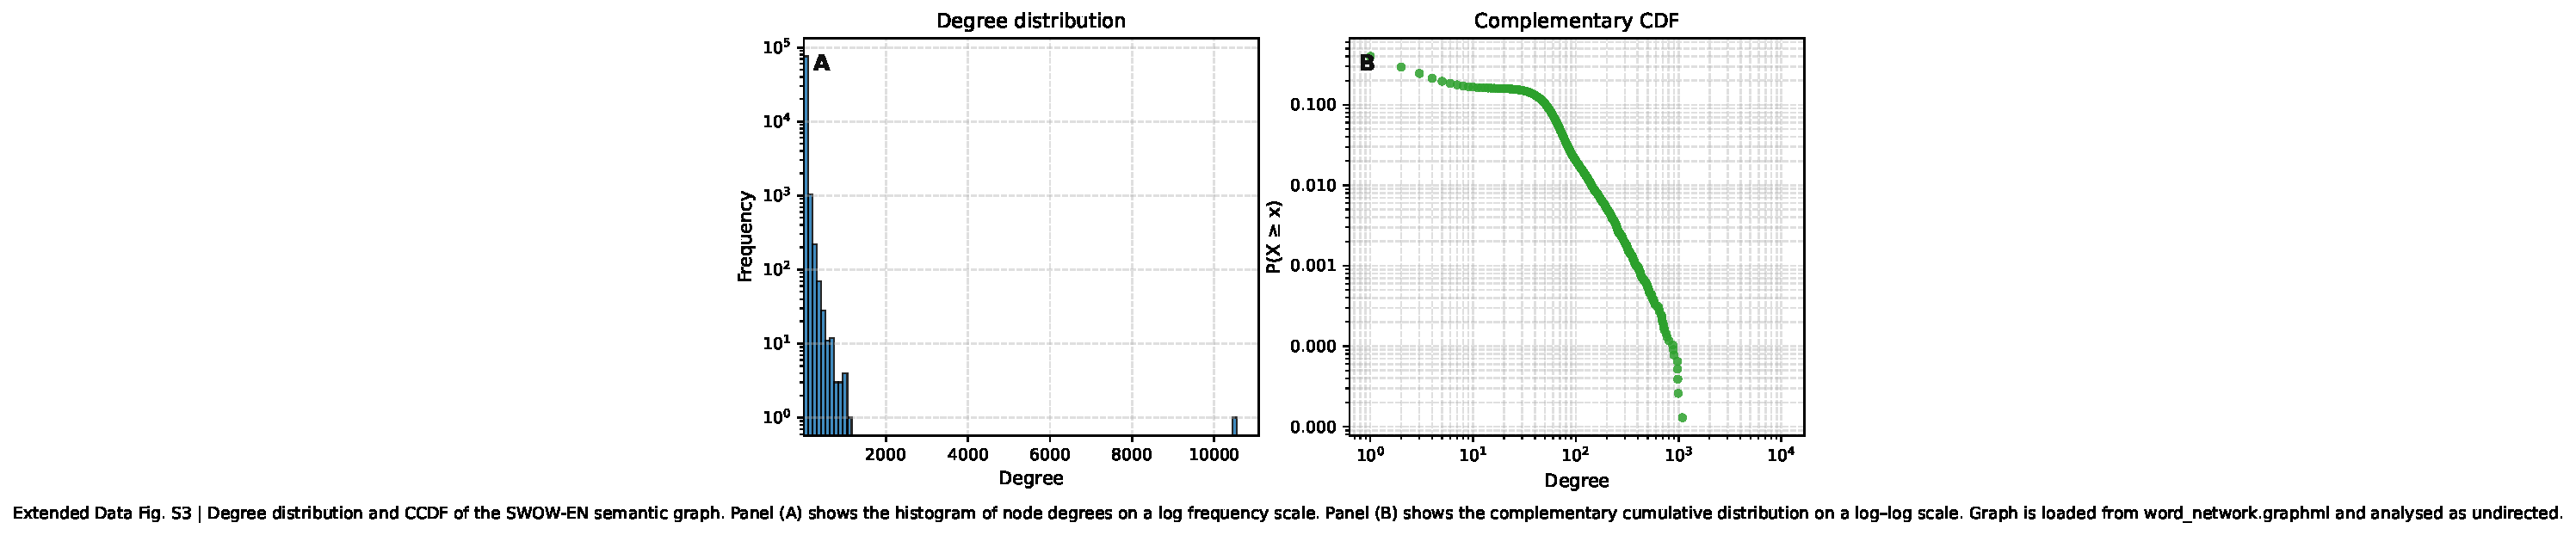
\includegraphics[width=\linewidth]{ext_S3_degree_distribution.pdf}
\caption{\textbf{Supplementary Fig. S3 | Degree distribution and CCDF of the SWOW-EN graph.} Left: log-scaled histogram of node degrees. Right: complementary cumulative distribution on log--log axes.}
\end{figure}

\begin{figure}[H]\centering
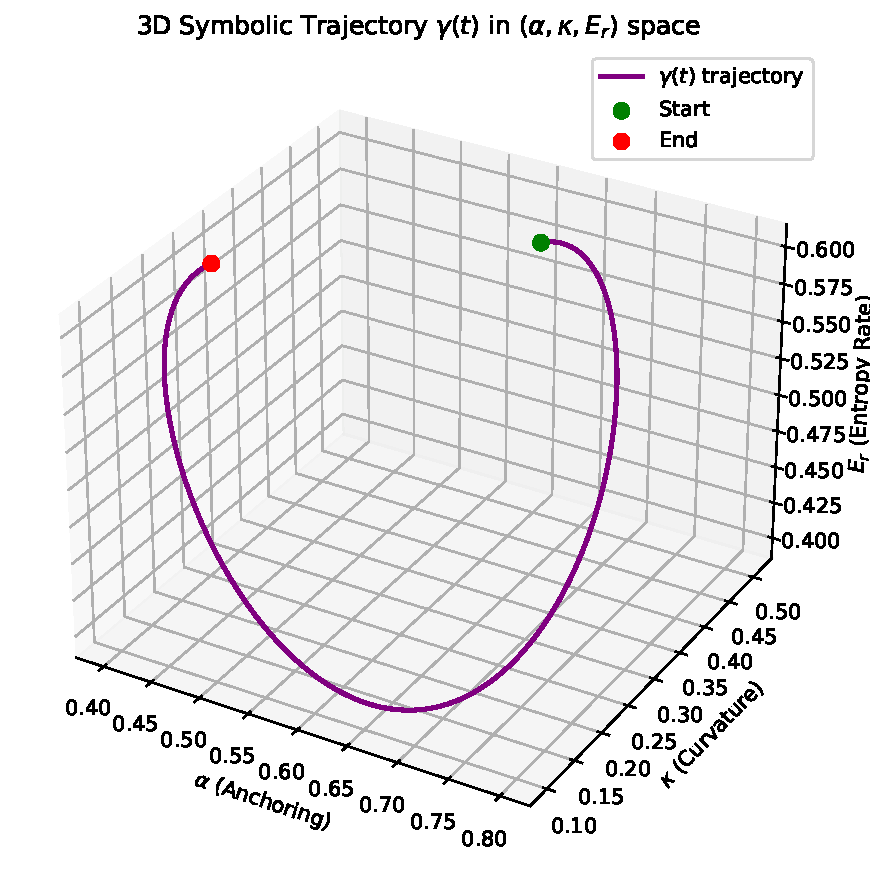
\includegraphics[width=\linewidth]{Fig_trajectory_3D.pdf}
\caption{\textbf{Supplementary Fig. S4 | Example 3D trajectory on the symbolic manifold.} Trajectory under varying $\beta$ and perturbations, illustrating regime transitions.}
\end{figure}

\begin{figure}[H]\centering
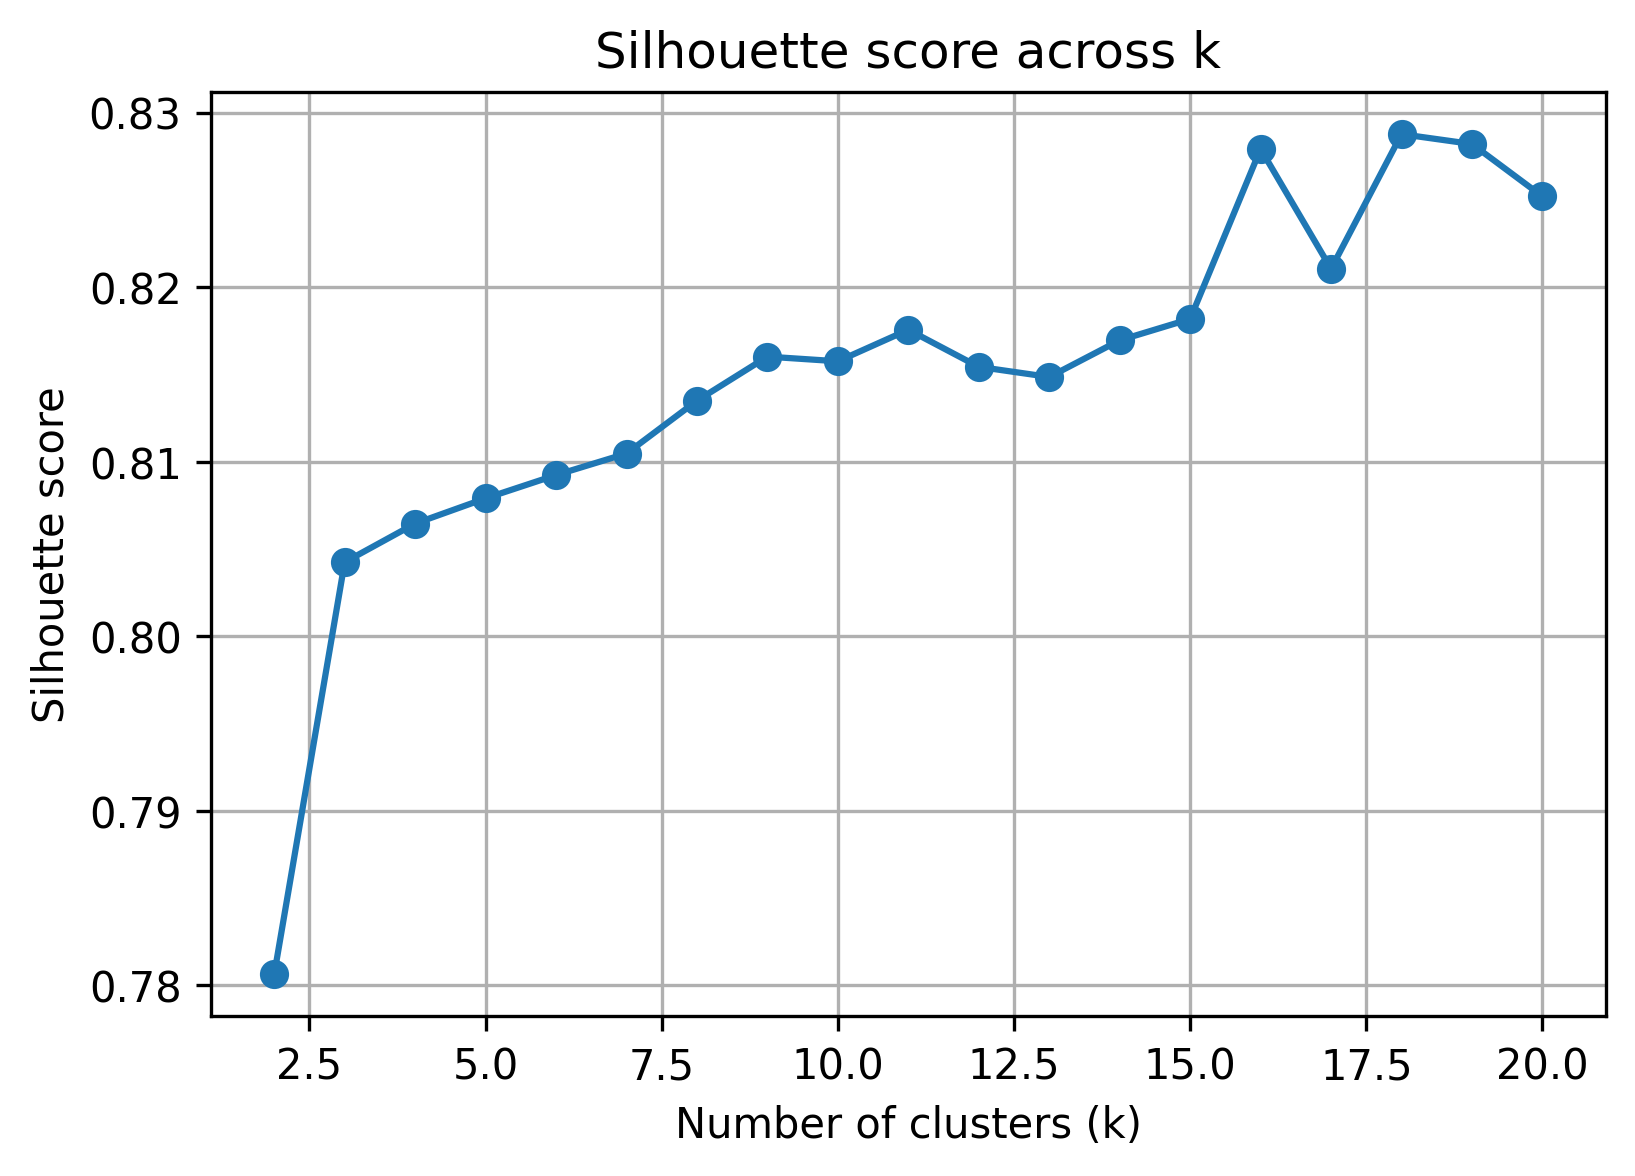
\includegraphics[width=\linewidth]{silhouette_scores.png}
\caption{\textbf{Supplementary Fig. S5 | Silhouette scores across $k$.} Internal separability for a range of cluster counts, complementing the HDBSCAN analysis.}
\end{figure}

\section*{Source Data}
CSV files with figure source data accompany this Supplementary Information: embedding projections (PCA/t-SNE/UMAP), entropy--curvature coordinates for real and null graphs, curvature distributions by $\alpha$, and cluster stability metrics.

\end{document}
